\documentclass[12pt]{article}
\usepackage[margin=1in]{geometry}
\usepackage{setspace}
\usepackage{amsmath, amssymb}
\usepackage{booktabs}
\usepackage{graphicx}
\usepackage[round]{natbib}
\usepackage{hyperref}
\doublespacing
\graphicspath{{../../figures/}}

\title{Neuro-Symbolic Search on a Hard Binary Linear System Family:\\
v6 Results, Negative Findings, and a Reinforcement Roadmap}
\author{neuroMCTS project}
\date{July 2026}

\begin{document}
\maketitle

\begin{abstract}
The v5 pipeline achieved near-perfect metrics on the original DNS family, but exact solvers closed the same instances in milliseconds, indicating an easy distribution rather than a solved problem. In this cycle, a market-split-style hard family was constructed at three sizes ($10 \times 25$, $20 \times 50$, $40 \times 100$; leak-free planted feasible instances and $\pm 1$-perturbed, CP-SAT-certified infeasible instances), and the v6 system was built for it: mixed-size training via segment softmax, size-invariant residual features, pump-trajectory and marginal-statistics features for the feasibility head, dense terminal rewards with a reverse curriculum, and a policy-guided complete backtracking stage. Timing is reported as a first-class metric throughout. Three results dominate. First, the hard family works as intended: heuristic baselines collapse (LP rounding to 2--27\% solution accuracy; LLL/BKZ misclassify up to 99\% of feasible instances), and exact solvers' runtimes grow by roughly three orders of magnitude (800--7{,}300$\times$) across the size sweep, with CP-SAT and SCIP failing to solve 9\% and 7\% of feasible $40 \times 100$ instances within a 60-second limit. Second, two honest negative results are documented with diagnostic evidence: AlphaZero-style self-play degraded test performance relative to the pre-trained policy (5.9\% vs.\ 9.6\% solution accuracy at $20 \times 50$), and the feasibility head converged to maximal uncertainty on fresh boundary instances, consistent with the NP-hardness of the distinction it was asked to make from static features. Third, a matched budget-scaling experiment shows sharply diminishing returns to search compute ($3.8\times$ time bought $+4$ points on identical instances), locating the binding constraint in search technology --- conflict learning and lattice-basis enumeration --- rather than in model capacity or budget, which defines the reinforcement roadmap for the next cycles.
\end{abstract}

\section{The Hard Family and Why the Old One Was Easy}

The construction and its rationale are documented in the companion note (\texttt{instance\_hardness\_and\_kernel\_pump.tex}); the essentials are repeated here. Feasible instances plant a solution of density exactly one half, so every right-hand-side entry concentrates at the row-sum midpoint and carries no directional information, following \citet{cornuejols1998market}. Infeasible instances perturb $k \in \{1,2,3\}$ rows of a planted right-hand side by $\pm 1$ --- the DNS dust-noise semantics --- and are retained only when CP-SAT \emph{proves} infeasibility. On the old family, 61.1\% of test instances were closed by symbolic rules before any neural inference; on the new family at $20 \times 50$, propagation closes nothing, the LP hard rule certifies 25 of 200 infeasible instances, and the kernel pump solves 44 of 800 feasible ones. Training data cannot be memorized: feasible training instances are generated fresh every epoch (certification-free by construction), and a documented false start --- a partial-flip ``gauge augmentation'' that turns out to leave the $\{0,1\}$ coefficient domain --- was replaced by the valid full-complement view for the pooled infeasible class, later superseded by fresh certified generation for the cheap sizes.

\section{The v6 System}

Relative to v5, the v6 system adds: (i) segment-softmax policy losses so batches mix instance sizes freely; (ii) row-degree-normalized residual buckets, making constraint features size-invariant; (iii) kernel-pump failure statistics (final/minimum normalized residual, mean fractionality, cycle rate) and assignment-marginal summary statistics as feasibility-head inputs; (iv) a focal feasibility loss; (v) per-epoch gradient-norm and policy-entropy logging; (vi) a value loss computed in the same sigmoid space the search reads, repairing a latent train/search mismatch; and (vii) two optional post-phases --- Plackett--Luce REINFORCE over DFS variable orderings, and a head-only feasibility fine-tune. Training proceeded as pre-training by masked-solution prediction (60 epochs, mask accuracy 50\% $\rightarrow$ 77.4\%), followed by 30 epochs of MCTS self-play over the three sizes.

\subsection{Reward starvation and its repair}

The first self-play attempt failed visibly in the new telemetry: solved-rate decayed from 0.072 toward 0.03, selection entropy declined from 3.74 to 1.86 over ten epochs, and the value loss collapsed to a constant --- the signature of a sparse-reward failure, since self-play almost never solved hard instances and the binary terminal reward was almost always zero. Three repairs were applied: a dense terminal reward ($1.0$ for exact solutions, else $0.5 \cdot \mathrm{sat}^2$ on the satisfied-row ratio, applied inside MCTS backups as well), a reverse curriculum that reveals a random fraction of the planted solution at episode start (cap $0.9$, annealed to zero by epoch 22), and the sigmoid-space value loss. Post-repair telemetry was healthy in the critical early phase: gradient norms fell from 8--18 to 0.2--2.3 within the first epochs, entropy stayed above 3.2 through the first third of the curriculum before declining as the policy committed, and full-difficulty solved-rate settled at 0.12--0.22 after the reveal reached zero.

\subsection{Negative result 1: self-play RL degraded test search}

Despite healthy training curves, the RL-trained policy \emph{underperformed} the pre-trained policy at test time (Table~\ref{tab:ckpt}): 5.88\% vs.\ 9.62\% solution accuracy at $20 \times 50$, with the DFS-ordering fine-tune recovering only part of the gap (7.50\%). The selection entropy's late decline (to 0.65 by epoch 30) indicates the policy committed to trajectory patterns that succeed near revealed solutions but do not transfer to full-difficulty search. The pre-trained checkpoint was therefore selected for final evaluation. The zero-shot strength of masked-prediction pre-training, combined with the failure of self-play to improve on it, mirrors the broader finding that learned components help most when embedded in exact search rather than when asked to drive open-loop construction \citep{gasse2019exact}.

\begin{table}[t]
\centering
\caption{Checkpoint comparison at $20 \times 50$ (1{,}000 test instances; identical search budgets, sims $=50$, DFS budget $40$k nodes). Times include LP/pseudo-inverse preprocessing.}
\label{tab:ckpt}
\begin{tabular}{lccc}
\toprule
Checkpoint & Feasibility acc.\ (\%) & Solution acc.\ (\%) & Avg.\ time (s) \\
\midrule
Pre-trained only (selected) & 82.50 & \textbf{9.62} & 7.12 \\
+ RL 30 epochs & 82.50 & 5.88 & 4.22 \\
+ DFS-ordering fine-tune & 82.50 & 7.50 & 7.55 \\
\bottomrule
\end{tabular}
\end{table}

\subsection{Negative result 2: the feasibility head cannot separate the boundary}

The v5 evaluation had already shown the head contributing zero correct rejections; v6 explains why, in two steps. First, training FeasAcc that peaked at 85.4\% (epoch 29; typical epochs sat at the 79.7\% all-feasible base rate) under the fresh-feasible/pooled-infeasible regime did not transfer to test (82.5\% $=$ symbolic rules alone): the head had learned to recognize the \emph{identity} of the 2{,}000 pooled infeasible instances --- a novelty-detection shortcut created by the data asymmetry. Second, after the asymmetry was repaired (fresh certified infeasible generation for $m \leq 20$) and the head alone was fine-tuned on balanced fresh data, the focal loss converged to its $p = 0.5$ fixed point ($\approx 0.173$) with accuracy pinned at 50\%: given frozen representations and pump statistics, fresh feasible and fresh barely-infeasible instances are indistinguishable. This is the expected shape of the problem --- a cheap static feature separating $\pm 1$-perturbed infeasible systems from feasible ones would contradict the hardness of the family --- and it redirects feasibility detection toward search-derived evidence (proof-based rejection), not classification.

\section{Results with Timing as a First-Class Metric}

\subsection{Baselines across the size sweep}

Table~\ref{tab:main} and Figure~\ref{fig:scaling} give the full picture. Exact solvers remain perfect through $20 \times 50$ but their runtimes grow by factors of 800--7{,}300 across the sweep, and at $40 \times 100$ CP-SAT leaves 73 of 800 feasible instances unsolved within its 60-second limit (SCIP: 54; Gurobi: 5). The heuristic baselines collapse on quality: LLL/BKZ declare 762--791 of 800 recoverable systems infeasible at $40 \times 100$, and LP rounding solves 2.25\%. The proposed pipeline (pre-trained policy $+$ pump $+$ MCTS $+$ budgeted DFS; the selected pre-trained checkpoint throughout) is saturated at $10 \times 25$ (99.30\% feasibility, 100.0\% solution accuracy at 1.50\,s), degrades to 9.62\% solution accuracy at $20 \times 50$, and at $40 \times 100$ (stratified 500-instance subset) reaches 80.20\% feasibility accuracy and 2.25\% solution accuracy at 25.0\,s per instance. The $40 \times 100$ stage attribution is stark: all nine solutions come from the kernel pump, the LP hard rule certifies one infeasible instance, and the MCTS and DFS stages contribute nothing within their budgets --- at this size the pipeline is effectively the pump plus an expensive failed search, while zero false negatives are retained. The sole bright spot is structural: the pump's per-instance cost stays in milliseconds at every size, so the one component built directly on the null-space formulation is also the only one whose cost curve is flat.

\begin{table}[t]
\centering
\caption{Hard-family test results across sizes (1{,}000 instances per size; proposed at $40\times100$ on a stratified 500-instance subset). Feas $=$ feasibility classification accuracy; Sol $=$ solution accuracy over feasible instances; $t$ $=$ average seconds per instance. Exact-solver time limit 60\,s.}
\label{tab:main}
\begin{tabular}{l ccc ccc ccc}
\toprule
& \multicolumn{3}{c}{$10 \times 25$} & \multicolumn{3}{c}{$20 \times 50$} & \multicolumn{3}{c}{$40 \times 100$} \\
\cmidrule(lr){2-4} \cmidrule(lr){5-7} \cmidrule(lr){8-10}
Method & Feas & Sol & $t$ (s) & Feas & Sol & $t$ (s) & Feas & Sol & $t$ (s) \\
\midrule
Gurobi MILP & 100 & 100 & 0.0023 & 100 & 100 & 0.028 & 100 & 99.4 & 1.88 \\
SCIP MILP & 100 & 100 & 0.0053 & 100 & 100 & 0.141 & 100 & 93.3 & 9.24 \\
CP-SAT & 100 & 100 & 0.0011 & 100 & 100 & 0.031 & 100 & 90.9 & 8.03 \\
LP relax (Gurobi) & 94.5 & 27.4 & 0.0005 & 82.5 & 7.6 & 0.0008 & 80.5 & 2.3 & 0.0020 \\
LP relax (SCIP) & 94.5 & 17.8 & 0.0017 & 82.5 & 5.5 & 0.0025 & 80.5 & 1.9 & 0.0063 \\
LLL & 76.0 & 70.0 & 0.0006 & 32.9 & 16.1 & 0.0029 & 20.9 & 1.1 & 0.024 \\
BKZ & 77.7 & 72.1 & 0.0010 & 36.4 & 20.5 & 0.0073 & 23.8 & 4.8 & 0.267 \\
\midrule
Proposed (v6) & 99.3 & 100.0 & 1.50 & 82.5 & 9.6 & 7.12 & 80.2 & 2.3 & 25.0 \\
\bottomrule
\end{tabular}
\end{table}

\begin{figure}[t]
\centering
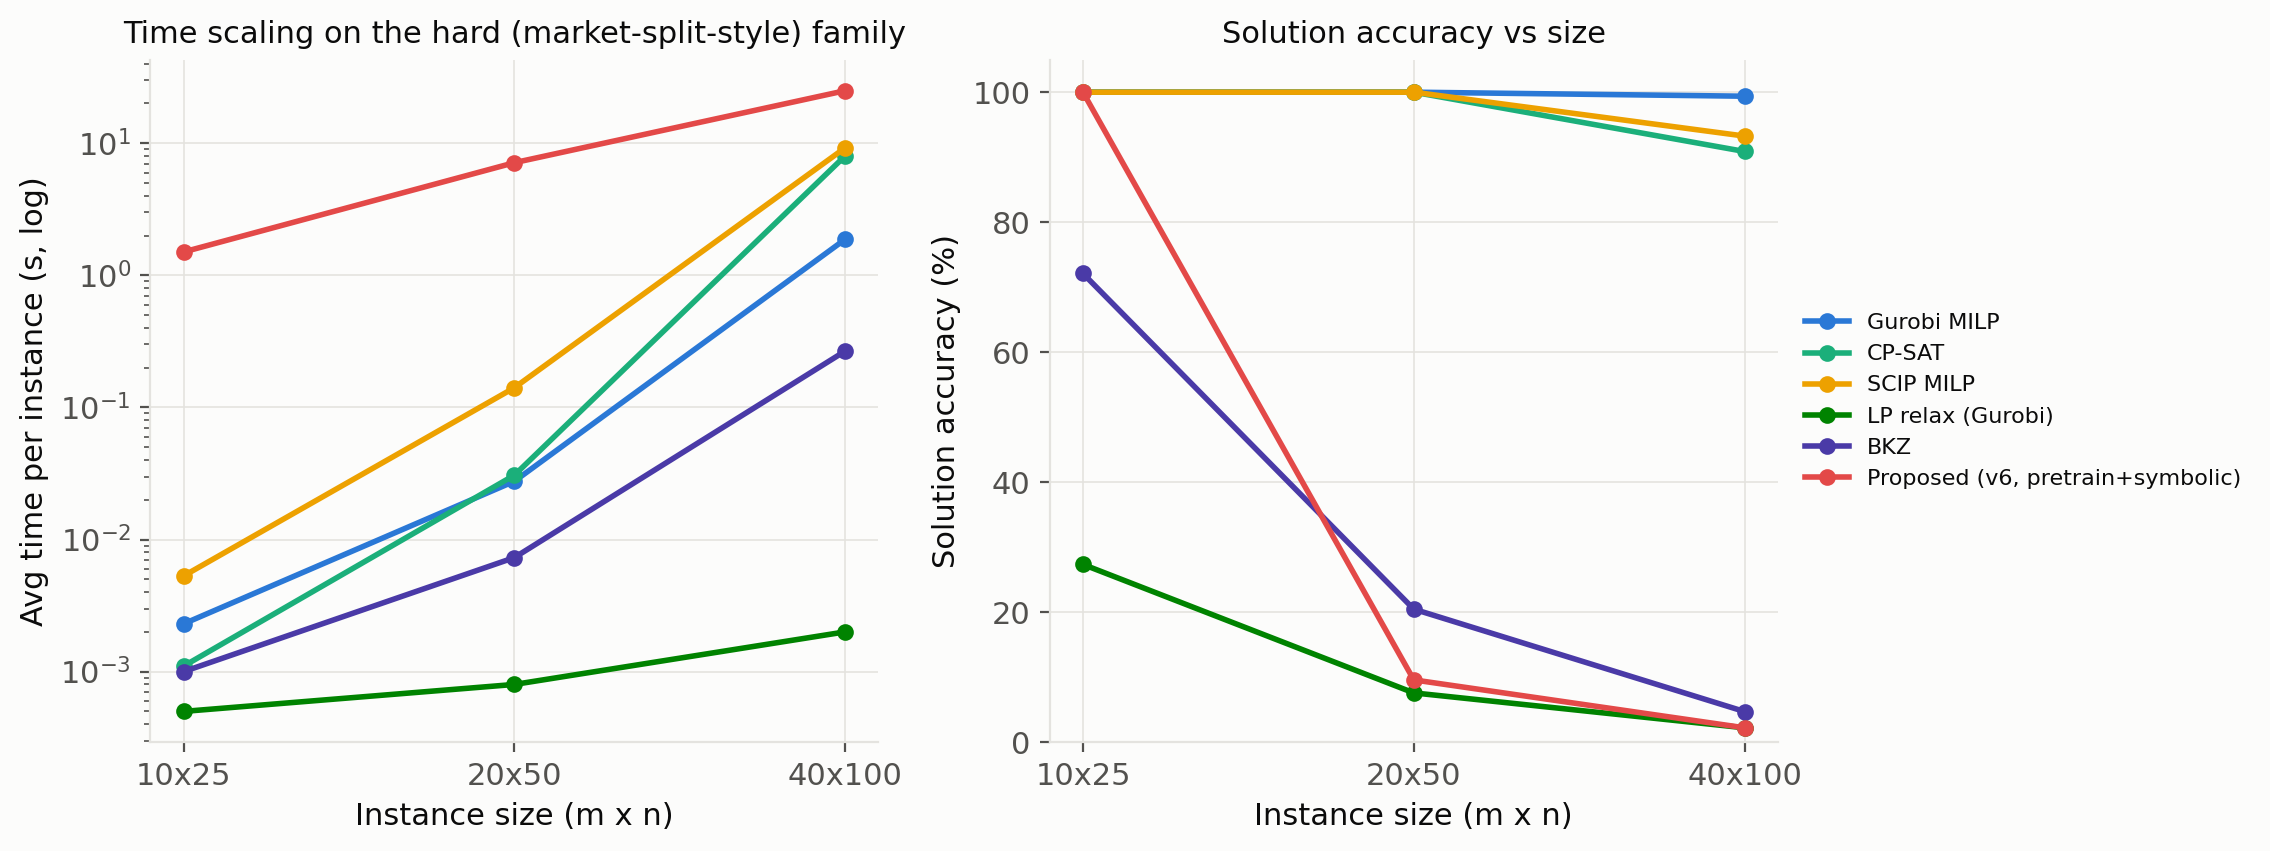
\includegraphics[width=\textwidth]{v6_time_accuracy_scaling.png}
\caption{Left: average per-instance time versus size (log scale). Exact-solver runtimes climb three to four orders of magnitude across the sweep while the proposed pipeline's time is dominated by its fixed search budget. Right: solution accuracy versus size.}
\label{fig:scaling}
\end{figure}

\subsection{Budget scaling: logarithmic returns}

On the same 100 feasible $20 \times 50$ instances evaluated under both budgets, quadrupling the search budget (sims $50 \rightarrow 200$, DFS $40$k $\rightarrow 200$k nodes; 7.3\,s $\rightarrow$ 28.2\,s per instance) raised the solved count from 9 to 13 (Figure~\ref{fig:budget}). CP-SAT solves the same instances at 100\% in 0.031\,s. The gap is therefore not compute but \emph{search technology}: conflict-driven learning, strong propagation, and restarts on the solver side; none of these exist in the current DFS, which rediscovers the same contradictions repeatedly under a static ordering.

\begin{figure}[t]
\centering
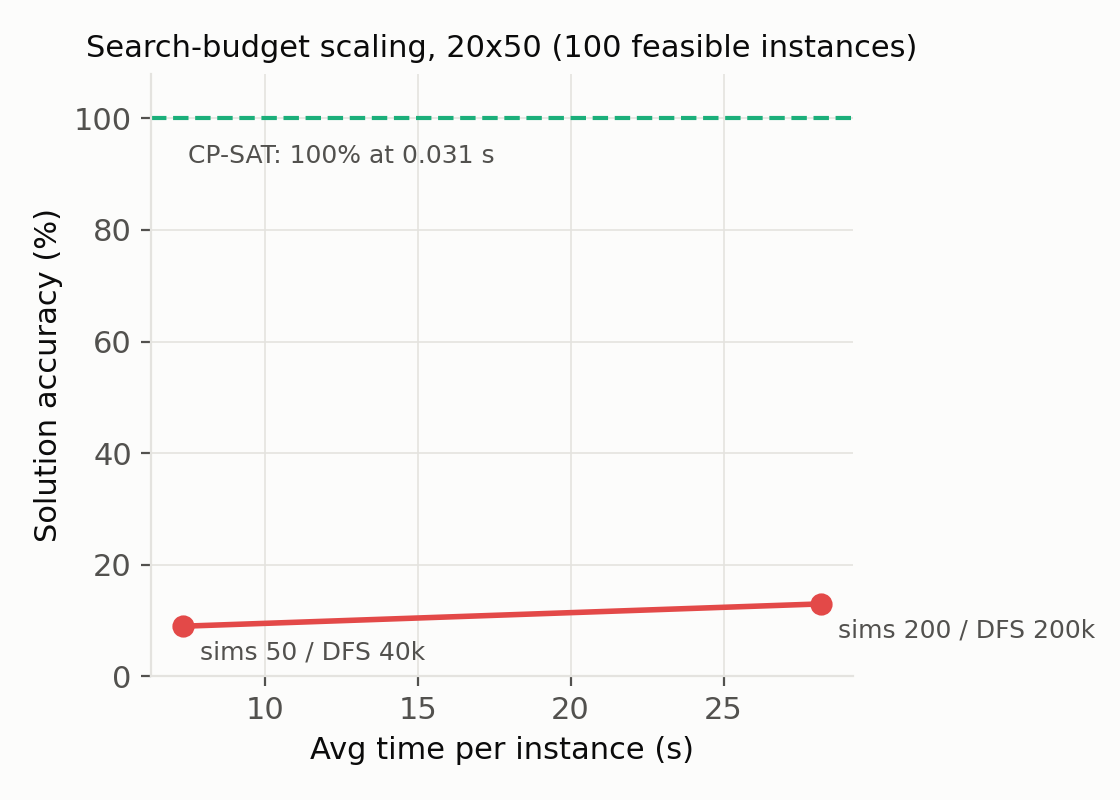
\includegraphics[width=0.6\textwidth]{v6_budget_scaling_20x50.png}
\caption{Solution accuracy versus average time as the search budget scales, $20 \times 50$. Returns are logarithmic; the binding constraint is search technology, not budget.}
\label{fig:budget}
\end{figure}

\section{Reinforcement Roadmap}

The evidence orders the next investments as follows.

\paragraph{1. Lattice-reformulated search (highest impact).} The only classical lineage that solves market-split-type systems at scale enumerates in an LLL-reduced kernel basis \citep{aardal2000market, wassermann2025market}. The pipeline currently uses the null space only for projection (the pump); branching in reduced-basis coefficient space --- with the learned model guiding enumeration order and bounds --- is the direct realization of the project's ``lattice $+$ learning'' novelty and the one change with headroom to rival exact solvers beyond $20 \times 50$.

\paragraph{2. Conflict learning in the DFS (best cost/benefit).} No-good recording, restarts, and periodic re-ranking of the branching order would import the mechanism that lets CP-SAT close these instances in milliseconds. This is a bounded engineering change to an existing component.

\paragraph{3. Reassigning the learned components.} Self-play construction failed here; imitation of strong-branching or CP-SAT decisions \citep{gasse2019exact, nair2020solving} inside the exact search, plus hardness prediction for budget allocation, are the literature-aligned roles. Feasibility detection should be proof-based (search-derived), not classified from static features.

\paragraph{Not worth reinforcing.} Additional self-play RL of the current form (empirically harmful), raw budget increases (logarithmic returns), and REINFORCE over DFS orderings at small budgets (flat reward $\approx 0.03$ across 10 epochs).

\section{Conclusion}

On a properly hard BLS family, the honest current standing is: the proposed pipeline dominates all inexact baselines at $10 \times 25$, loses to lattice heuristics at $20 \times 50$ on solution accuracy while retaining zero false negatives, and --- like every non-exact method tested --- is far from the exact solvers wherever they finish within their time limit. The exact solvers' own runtime explosion across the sweep (and their first failures at $40 \times 100$) confirms that the target problem class eventually escapes them, which keeps the research question alive; the budget-scaling experiment says the way to that regime is smarter search, not more of the current search. Two negative results --- self-play degradation and the feasibility head's convergence to indifference --- are reported as findings with diagnostic evidence, and the roadmap above converts them into the next cycle's design.

\begin{thebibliography}{9}
\bibitem[Aardal et al.(2000)]{aardal2000market}
Aardal, K., Bixby, R. E., Hurkens, C. A. J., Lenstra, A. K., \& Smeltink, J. W. (2000). Market split and basis reduction: Towards a solution of the Cornu\'ejols--Dawande instances. \emph{INFORMS Journal on Computing, 12}(3), 192--202.

\bibitem[Cornu\'ejols \& Dawande(1998)]{cornuejols1998market}
Cornu\'ejols, G., \& Dawande, M. (1998). A class of hard small 0--1 programs. In \emph{Integer Programming and Combinatorial Optimization} (pp. 284--293). Springer.

\bibitem[Gasse et al.(2019)]{gasse2019exact}
Gasse, M., Ch\'etelat, D., Ferroni, N., Charlin, L., \& Lodi, A. (2019). Exact combinatorial optimization with graph convolutional neural networks. \emph{Advances in Neural Information Processing Systems, 32}.

\bibitem[Nair et al.(2020)]{nair2020solving}
Nair, V., Bartunov, S., Gimeno, F., von Glehn, I., Lichocki, P., Lobov, I., \ldots{} \& Zwols, Y. (2020). Solving mixed integer programs using neural networks. \emph{arXiv preprint arXiv:2012.13349}.

\bibitem[Wassermann(2025)]{wassermann2025market}
Wassermann, A. (2025). Solving the market split problem with lattice enumeration. \emph{arXiv preprint arXiv:2508.08702}.
\end{thebibliography}

\end{document}
